\chapter{Prerequisites}
\begin{chapquote}{H.G. Rice [1953], \textit{paraphrased by Anders Moller}}
  ``Everything interesting about the behaviour of programs is
  undecidable.''
\end{chapquote}

The goal of \textit{static program analysis} is to verify certain
\textsl{properties} (or \textsl{behaviours}, or
\textsl{specifications}, or \textsl{statements}, ...) of the target
program \textbf{without its execution}.

For program \textsl{P} and property \textsl{S},

\begin{itemize}
\item $ \SEM{P} $: Formal semantics of program \textsl{P}.

\item \textsl{S}: Semantic properties that we're interested in. This
  could be defined in various level, such as ``Division-by-zero will
  \textbf{never} occur'' or ``The variable \textit{i} is always 3''.

\item Soundness: $ analysis(P) = true \implies S $

\item Completeness: $ S \implies analysis(P) = true $

\item Scalability: Time complexity.
\end{itemize}


\textbf{No analysis} can be sound and complete at the same time. If an
analysis is sound, then it is also incomplete, and vice versa.

%%%%%%%%%%%%%%%%%%%%%%%%%%%%%%%%%%%%%%%%%%%%%%%%%%%%%%%%%%%%%%%%%%%%%%%%%%%%%%%%%%%%%%%%%%%%%%%%%%%%
\newpage
\section{Relation Theory}
This note originates from
Proofwiki\footnote{https://proofwiki.org}.

\subsection{Relation}

Let $S \times T$ be the Cartesian product of two sets $S$ and $T$.A
\textbf{relation} on $S \times T$ is an ordered triple
$ \mathcal{R} = (S, T, R) $ where $R \subseteq S \times T$ is a subset
of the Cartesian product of $S$ and $T$.

What this means is that a \textbf{relation} \textit{relates} (certain)
elements of one set or class $S$ with (certain) elements of another,
$T$. Not all elements of $S$ need to be related to every (or even any)
element of $T$.

\paragraph{Notation}

If $(x, y)$ is an ordered pair such that $(x, y) \in \mathcal{R}$, we
use the notation: $ s \mathcal{R} t$ or $ \mathcal{R}(s, t)$ and can
say:
\begin{itemize}
\item $s$ \textbf{bears} $\mathcal{R}$ to $t$
\item $s$ \textbf{stands in} the relation $\mathcal{R}$ to $t$
\end{itemize}

\paragraph{General Definition}

Let
$\mathbb{S} = \displaystyle \prod_{i=1}^n S_i = S_1 \times S_2 \times ... \times S_n $
be the Cartesian product on $n$ sets $S_1, ..., S_n$.

An \textbf{$n$-ary relation on} $\mathbb{S}$ is an ordered
$n+1$-tuple $\mathcal{R}$ defined as

\begin{math}
  \begin{array}{c}
    \\
    \mathcal{R} := (S_1, S_2, ..., S_n, R)\\
    \\
  \end{array}
\end{math}

where $\mathcal{R}$ is an arbitrary subset
$\mathcal{R} \subseteq \mathbb{S}$.

To indicate that $(s_1, s_2, ..., s_n) \in R$, we write:
$\mathcal{R}(s_1, s_2, ..., s_n)$


\paragraph{Unary Relation}

As a special case of an $n$-ary relation on $S$, note that when $n=1$
we define a \textbf{unary relation} on $S$ as
$\mathcal{R} \subseteq S$. That is, a \textbf{unary relation} is a
subset of $S$.



\subsection{Domain}
\label{sec:domain}

Let $\mathcal{R} \subseteq S \times T$ be a relation. The
\textbf{domain} of $\mathcal{R}$ is defined and denoted as:

\begin{math}
  \begin{array}{c}
    \\
    \mathtt{Dom}(\mathcal{R}) := \{ s \in S: \exists t \in T: (s, t) \in \mathcal{R} \}\\
    \\
  \end{array}
\end{math}

\paragraph{General Definition}

Let $\displaystyle \prod_{i=1}^n S_i$ be the Cartesian product of sets
$S_1$ to $S_n$. Let
$\mathcal{R} \subseteq \displaystyle \prod_{i=1}^n S_i$ be an $n$-ary
relation on $\displaystyle \prod_{i=1}^n S_i$.

The \textbf{domain of $\mathcal{R}$} is the set defined as:

\begin{math}
  \begin{array}{c}
    \\
    \mathtt{Dom}(\mathcal{R}) := \{ (s_1, s_2, ..., s_{n-1}) \in \displaystyle \prod_{i=1}^{n-1} S_i : \exists s_n \in S_n : (s_1, s_2, ..., s_n) \in \mathcal{R} \}\\
    \\
  \end{array}
\end{math}

The concept is usually encountered when $\mathcal{R}$ is an
endorelation on $S$:

\begin{math}
  \begin{array}{c}
    \\
    \mathtt{Dom}(\mathcal{R}) := \{ (s_1, s_2, ..., s_{n-1}) \in S^{n-1} : \exists s_n \in S : (s_1, s_2, ..., s_n) \in \mathcal{R} \}\\
    \\
  \end{array}
\end{math}


\subsection{Codomain}
\label{sec:codomain}

The \textbf{codomain} of a relation $\mathcal{R} \subseteq S \times T$
is the set $T$. It can be denoted as $\mathtt{Cdm}(\mathcal{R})$.


\subsection{Image}
\label{sec:image}

Let $\mathcal{R} \subseteq S \times T$ be a relation. The
\textbf{image} of $\mathcal{R}$ is the set:

\begin{math}
  \begin{array}{c}
    \\
    \mathtt{Img}(\mathcal{R}) := \mathcal{R}[S] = \{ t \in T: \exists s \in S: (s, t) \in \mathcal{R} \}\\
    \\
  \end{array}
\end{math}

\paragraph{General Definition}

Let $\displaystyle \prod_{i=1}^n S_i$ be the Cartesian product of sets
$S_1$ to $S_n$. Let
$\mathcal{R} \subseteq \displaystyle \prod_{i=1}^n S_i$ be an $n$-ary
relation on $\displaystyle \prod_{i=1}^n S_i$.

The \textbf{image of $\mathcal{R}$} is the set defined as:

\begin{math}
  \begin{array}{c}
    \\
    \mathtt{Img}(\mathcal{R}) := \{ s_n \in S_n: \exists (s_1, s_2, ..., s_{n-1} \in \displaystyle \prod_{i=1}^{n-1} S_i: (s_1, s_2, ..., s_n) \in \mathcal{R} \}\\
    \\
  \end{array}
\end{math}

The concept is usually encountered when $\mathcal{R}$ is an
endorelation on $S$:

\begin{math}
  \begin{array}{c}
    \\
    \mathtt{Img}(\mathcal{R}) := \{ s_n \in S: \exists (s_1, s_2, ..., s_{n-1}) \in S^{n-1}: (s_1, s_2, ..., s_n) \in \mathcal{R} \}\\
    \\
  \end{array}
\end{math}


\subsection{Endorelation}
\label{sec:endorelation}
Let $S \times S$ be the Cartesian product of a set or class $S$ with
itself. Let $\mathcal{R}$ be a \textbf{relation} on $S \times S$. Then
$\mathcal{R}$ is referred to as an \textbf{endorelation on} $S$.


The term \textbf{endorelation} is rarely seen. Once it is established
that the \textit{domain} and \textit{codomain} of a given relation are
the \textbf{same set}, further comment is rarely needed.


An \textbf{endorelation} is also called a \textbf{relation in} $S$, or
a \textbf{relation on} $S$. The latter term is discouraged, though,
because it can also mean a left-total relation, and confusion can
arise.

Some sources use the term \textbf{binary relation} exclusively to
refer to a \textbf{binary endorelation}.


\subsection{Many-to-One Relation}
\label{sec:many-to-one}

A relation $\mathcal{R} \subseteq S \times T$ is \textbf{many-to-one}
if and only if:

\begin{math}
  \begin{array}{c}
    \\
    \forall x \in \mathtt{Dom}(\mathcal{R}): \forall y_1, y_2 \in \mathtt{Cdm}(\mathcal{R}): (x, y_1) \in \mathcal{R} \land (x, y_2) \in \mathcal{R} \implies y_1 = y_2 \\
    \\
  \end{array}
\end{math}

That is, every element of the domain of $\mathcal{R}$ relates to no
more than one element of its codomain.

\subsection{One-to-Many Relation}
\label{sec:one-to-many}

A relation $\mathcal{R} \subseteq S \times T$ is \textbf{one-to-many}
if and only if:

\begin{math}
  \begin{array}{c}
    \\
    \forall y \in \mathtt{Img}(\mathcal{R}): (x_1, y) \in \mathcal{R} \land (x_2, y) \in \mathcal{R} \implies x_1 = x_2 \\
    \\
  \end{array}
\end{math}

That is, every element of the image of $\mathcal{R}$ relates to by
exactly one element of its domain. Note that the condition concerns
the elements in the \textit{image}, not the
\textit{codomain}\footnote{Thus, a one-to-many relation may leave some
  element(s) of the codomain unrelated}.

Also called as \textit{injective relation}\ref{sec:injection}.

\subsection{One-to-One Relation}
\label{sec:one-to-one}

A relation $\mathcal{R} \subseteq S \times T$ is \textbf{one-to-one}
if it is both many-to-one and one-to-many. That is, every element of
the domain of $\mathcal{R}$ relates to no more than one element of its
codomain, and every element of the image is related to by exactly one
element of its domain.


\subsection{Left-Total Relation}
\label{sec:left-total}

Let $S$ and $T$ be sets, and $\mathcal{R} \subseteq S \times T$ be a
relation in $S$ to $T$. Then $\mathcal{R}$ is \textbf{left-total} if
and only if:

\begin{math}
  \begin{array}{c}
    \\
    \forall s \in S: \exists t \in T: (s, t) \in \mathcal{R} \\
    \\
  \end{array}
\end{math}

That is, if and only if every element of $S$ relates to some element
of $T$, i.e., the domain of $\mathcal{R}$ equals to $S$.


\subsection{Right-Total Relation}
\label{sec:right-total}

Let $S$ and $T$ be sets, and $\mathcal{R} \subseteq S \times T$ be a
relation in $S$ to $T$. Then $\mathcal{R}$ is \textbf{right-total} if
and only if:

\begin{math}
  \begin{array}{c}
    \\
    \forall t \in T: \exists s \in S: (s, t) \in \mathcal{R} \\
    \\
  \end{array}
\end{math}

That is, if and only if every element of $T$ relates to by some
element of $S$, i.e., the image of $\mathcal{R}$ equals to $T$.


\subsection{Mapping}
\label{sec:mapping}

Let $S$ and $T$ be sets, and $S \times T$ be their Cartesian product.


\paragraph{Definition 1}

A \textbf{mapping} from $S$ to $T$ is a binary relation on
$S \times T$ which associates each element of $S$ with exactly one
element of $T$.

\paragraph{Definition 2}

A \textbf{mapping $f$ from $S$ to $T$}, denoted $f: S \to T$, is a
relation $f = (S, T, G)$ where $G \subseteq S \times T$ such that:

\begin{math}
  \begin{array}{l}
    \\
    \forall x \in S: \forall y_1, y_2 \in T: (x, y_1) \in G \land (x, y_2) \in G \implies y_1 = y_2 \\
    \text{and} \\
    \forall x \in S: \exists y in T: (x, y) \in G \\
    \\
  \end{array}
\end{math}

\paragraph{Definition 3}

A \textbf{mapping $f$ from $S$ to $T$}, denoted $f: S \to T$, is a
relation $f = (S, T, R)$ where $R \subseteq S \times T$ such that:

\begin{math}
  \begin{array}{l}
    \\
    \forall (x_1, y_1), (x_2, y_2) \in \mathcal{R}: y_1 \neq y_2 \implies x_1, x_2 \\
    \text{and} \\
    \forall x \in S: \exists y \in T: (x, y) \in \mathcal{R} \\
    \\
  \end{array}
\end{math}

\paragraph{Definition 4}

A \textbf{mapping from $S$ to $T$} is a relation on $S \times T$ which is:

\begin{itemize}
\item Many-to-one
\item Left-total, that is, defined for all elements in $S$
\end{itemize}

\paragraph{Self-Map}
\label{sec:self-map}

Let $S$ be a set. A \textbf{self-map on $S$} is a \textbf{mapping}
from $S$ to itself: $f: S \to S$.

\paragraph{Defined}
\label{sec:defined}

A mapping $f \subseteq S \times T$ is \textbf{defined} at $x \in S$ if
and only if:

\begin{math}
  \begin{array}{c}
    \\
    \exists y \in T: (x, y) \in f\\
    \\
  \end{array}
\end{math}

If for some $x \in S$, one has:

\begin{math}
  \begin{array}{c}
    \\
    \forall y \in T: (x, y) \notin f\\
    \\
  \end{array}
\end{math}

then $f$ is \textbf{not defined} or \textbf{undefined} at $x$, and
indeed, $f$ is not technically a mapping at all.


\subsection{Injection}
\label{sec:injection}

A mapping $f$ is an \textbf{injection} or \textbf{injective} if and
only if:

\begin{math}
  \begin{array}{c}
    \\
    \forall x_1, x_2 \in \mathtt{Dom}(f): f(x_1) = f(x_2) \implies x_1 = x_2 \\
    \\
  \end{array}
\end{math}

That is, an injection is a mapping such that the output
\textit{uniquely determines} its input.

\subsection{Surjection}
\label{sec:surjection}

Let $S$ and $T$ be sets and $f : S \to T$ be a mapping from $S$ to
$T$. $f$ is a \textbf{subjection} if and only if

\begin{math}
  \begin{array}{c}
    \\
    \forall y \in T: \exists x \in \mathtt{Dom}(f) : f(x) = y\\
    \\
  \end{array}
\end{math}

That is, if and only if $f$ is right-total.

Also called as \textbf{onto mapping}, or just \textbf{onto}\footnote{A
  mapping which is not surjective is hence described as \textbf{into}}.


\subsection{Bijection}
\label{sec:bijection}

A mapping $f: S \to T$ is a \textbf{bijection} if and only if both
\begin{itemize}
\item $f$ is an injection
\item $f$ is a surjection
\end{itemize}



\subsection{Symmetry}
\label{sec:symmetry}
The word \textit{symmetry} comes from Greek symmetria meaning
\textbf{measure together}.

\paragraph{Definition}

Let $\mathcal{R} \subseteq S \times S$ be a relation in $S$.

\subsubsection{Symmetric}

$\mathcal{R}$ is \textbf{symmetric} if and only if

\begin{math}
  \begin{array}{c}
    \\
    (x, y) \in \mathcal{R} \implies (y, x) \in \mathcal{R}\\
    \\
  \end{array}
\end{math}


\subsubsection{Asymmetric}

$\mathcal{R}$ is \textbf{asymmetric} if and only if

\begin{math}
  \begin{array}{c}
    \\
    (x, y) \in \mathcal{R} \implies (y, x) \notin \mathcal{R}\\
    \\
  \end{array}
\end{math}


\subsubsection{Antisymmetric}

$\mathcal{R}$ is \textbf{antisymmetric} if and only if

\begin{math}
  \begin{array}{ll}
    \\
    &(x,y) \in \mathcal{R} \land (y, x) \in \mathcal{R} \implies x = y\\
    \text{i.e., } & \{(x, y), (y, x) \} \subseteq \mathcal{R} \implies x = y \\
    \\
  \end{array}
\end{math}


Antisymettry eliminates uncertain cases when both $a$ precedes $b$ and
$b$ precedes $a$.

\subsubsection{Non-symmetric}

$\mathcal{R}$ is \textbf{non-symmetric} if and only if it is neither
\textit{symmetric} nor \textit{asymmetric}.

\paragraph{Antisymmetric and Asymmetric}

Note the difference between:
\begin{itemize}
\item An \textit{asymmetric relation}, in which the fact that
  $(x, y) \in \mathcal{R}$ means that $(y, x)$ is defintely
  \textbf{not} in $\mathcal{R}$
\item An \textit{antisymmetric relation}, in which there \textit{may}
  be instances of both $(x, y) \in \mathcal{R}$ and
  $(y, x) \in \mathcal{R}$, but if there are, then it means that $x$
  and $y$ have to be the same object.
\end{itemize}


\subsection{Reflexivity}
\label{sec:reflexivity}

\paragraph{Definition}

Let $\mathcal{R} \subseteq S \times S$ be a relation in $S$.

\subsubsection{Reflexive}

$\mathcal{R}$ is \textbf{reflexive} if and only if

\begin{math}
  \begin{array}{c}
    \\
    \forall x \in S : (x, x) \in \mathcal{R} \\
    \\
  \end{array}
\end{math}



\subsubsection{Coreflexive}

$\mathcal{R}$ is \textbf{coreflexive} if and only if

\begin{math}
  \begin{array}{c}
    \\
    \forall x, y \in S : (x, y) \in \mathcal{R} \implies x = y\\
    \\
  \end{array}
\end{math}



\subsubsection{Antireflexive}

$\mathcal{R}$ is \textbf{antireflexive} if and only if

\begin{math}
  \begin{array}{c}
    \\
    \forall x \in S: (x, x) \notin \mathcal{R}\\
    \\
  \end{array}
\end{math}



\subsubsection{Non-reflexive}

$\mathcal{R}$ is \textbf{non-reflexive} if and only if it is neither
\textit{reflexive} nor \textit{antireflexive}.


\subsection{Transitivity}
\label{sec:transitivity}

\paragraph{Definition}

Let $\mathcal{R} \subseteq S \times S$ be a relation in $S$.

\subsubsection{Transitive}

$\mathcal{R}$ is \textbf{transitive} if and only if

\begin{math}
  \begin{array}{ll}
    \\
    & (x, y) \in \mathcal{R} \land (y, z) \in \mathcal{R} \implies (x, z) \in \mathcal{R}\\
    \text{i.e., } & \{(x, y), (y, z)\} \subseteq \mathcal{R} \implies (x, z) \in \mathcal{R} \\
    \\
  \end{array}
\end{math}


\subsubsection{Antitransitive}

$\mathcal{R}$ is \textbf{antitransitive} if and only if

\begin{math}
  \begin{array}{ll}
    \\
    & (x, y) \in \mathcal{R} \land (y, z) \in \mathcal{R} \implies (x, z) \notin \mathcal{R}\\
    \text{i.e., }& \{ (x, y), (y, z) \} \subseteq \mathcal{R} \implies (x, z) \notin \mathcal{R}\\
    \\
  \end{array}
\end{math}



\subsubsection{Non-transitive}

$\mathcal{R}$ is \textbf{non-transitive} if and only if it is neither
\textit{transitive} nor \textit{antitransitive}.


\subsubsection{Transitive Closure}
\label{sec:transitive-closure}

Let $\mathcal{R}$ be a relation on a set $S$. The \textbf{transitive
  closure of $\mathcal{R}$} is defined as the smallest transitive
relation on $S$ which contains $\mathcal{R}$ as a subset.

Or, the \textbf{transitive closure of $\mathcal{R}$} is defined as the
intersection of all transitive relations on $S$ which contains
$\mathcal{R}$.

Or, the \textbf{transitive closure of $\mathcal{R}$} is the relation
$\mathcal{R}^+$ defined as follows:


\begin{math}
  \begin{array}{c}
    \\
    \forall x, y \in S, x \mathcal{R}^+ y \iff \exists n \in \mathbb{N}_{>0} : \exists s_0, s_1, ..., s_n \in S: s_0 = x, s_n = y \\
    \\
    s_0 \mathcal{R} s_1\\
    s_1 \mathcal{R} s_2\\
    \vdots\\
    s_{n-1} \mathcal{R} s_n \\
    \\
  \end{array}
\end{math}


\subsection{Total Relation}
\label{sec:total-relation}

Let $\mathcal{R} \subseteq S \times S$ be a relation on a set
$S$. Then $\mathcal{R}$ is defined as \textbf{total} if and only if:

\begin{math}
  \begin{array}{c}
    \\
    \forall a, b \in S : (a, b) \in \mathcal{R} \lor (b, a) \in \mathcal{R} \\
    \\
  \end{array}
\end{math}

That is, if and only if every pair of elements is related.

Also called as \textbf{strictly connected}, or \textbf{complete
  relation}.

\subsection{Connected Relation}
\label{sec:connected-relation}

Let $\mathcal{R} \subseteq S \times S$ be a relation on a set
$S$. Then $\mathcal{R}$ is \textbf{connected} if and only if:

\begin{math}
  \begin{array}{c}
    \\
    \forall a, b \in S: a \neq b \implies (a, b) \in \mathcal{R} \lor (b,a) \in \mathcal{R} \\
    \\
  \end{array}
\end{math}


That is, if and only if every pair of \textit{distinct} elements is
related.


A relation having the \textbf{connexivity} means that any pair of
elements in the set of the relation are comparable under the
relation. This also means that the set can be diagrammed as a line of
elements, giving it the name \textit{linear}. The connexivity also
implies reflexivity, i.e., $a \leq a$.

Also called as \textbf{weakly connected}, while \textit{strictly
  connected} refers to \textit{total
  relation}\ref{sec:total-relation}.


\subsection{Relation Compatible with Operation}
\label{sec:compatibility}

Let $(S, \circ)$ be a magma. Let $\mathcal{R}$ be a relation on $S$.

Then $\mathcal{R}$ is \textbf{compatible with $\circ$} if and only if:

\begin{itemize}
\item $\forall x, y, z \in S: x \mathcal{R} y \implies (x \circ z) \mathcal{R} (y \circ z)$
\item $\forall x, y, z \in S: x \mathcal{R} y \implies (z \circ x) \mathcal{R} (z \circ y)$
\end{itemize}


\subsection{Relational Structure}
\label{sec:relational-structure}

A \textbf{relational structure} is an ordered pair $(S, \mathcal{R})$,
where:

\begin{itemize}
\item $S$ is a set
\item $\mathcal{R}$ is an endorelation\ref{sec:endorelation} on $S$
\end{itemize}

Also called as a \textbf{relational system}.



%%%%%%%%%%%%%%%%%%%%%%%%%%%%%%%%%%%%%%%%%%%%%%%%%%%%%%%%%%%%%%%%%%

\subsection{Binary Operation}
\label{sec:binary-operation}

A \textbf{binary operation} is a mapping $\circ$ from the Cartesian
product of two sets $S \times T$ to a universe $\mathbb{U}$:

\begin{math}
  \begin{array}{c}
    \\
    \circ: S \times T \to \mathbb{U} : \circ(s, t) = y \in \mathbb{U} \\
    \\
  \end{array}
\end{math}

If $S = T$ , then $\circ$ can be referred to as a \textbf{binary
  opeation on $S$}.

Some authors specify that a binary operation is defined such that
\textit{codomain} of $\circ$ is the same underlying set as that which
forms the \textit{domain}, that is: $\circ: S \times S \to S$.


\subsection{Algebraic Structure}
\label{sec:algebraic-structure}

An \textbf{algebraic structure} is an ordered tuple:

\begin{math}
  \begin{array}{c}
    (S, \circ_1, \circ_2, ..., \circ_n)
  \end{array}
\end{math}

where $S$ is a set which has one or more binary operations
$\circ_1, \circ_2, ..., \circ_n$ defined on all the elements of
$S \times S$.

An algebraic structure with one (binary) operation is thus an ordered
pair which can be denoted as $(S, \circ)$ or $(T, *)$ or
$\pair{S, \circ}$, and so on.

The set $S$ is called \textbf{underlying set}.


\subsection{Closure}
\label{sec:closure}

Let $(S, \circ)$ be an algebraic structure. Then $S$ has the property
of \textbf{closure under $\circ$} if and only if:

\begin{math}
  \begin{array}{c}
    \\
    \forall (x, y) \in S \times S : x \circ y \in S\\
    \\
  \end{array}
\end{math}


$S$ is said to be \textbf{closed under $\circ$}, or just that
$(S, \circ)$ \textbf{is closed}.

\subsection{Magma}
\label{sec:magma}

A \textbf{magma} is an algebraic structure $(S, \circ)$ such that $S$
is closed unser $\circ$.

That is, a magma is a pair $\pair{S, \circ}$ where:

\begin{itemize}
\item $S$ is a set
\item $\circ: S \times S \to S $ is a binary operation on $S$.
\end{itemize}




\subsection{Commutativity}
\label{sec:commutativity}

Let $(S, \circ)$ be an algebraic structure. Then $\circ$ is
\textbf{commutative on $S$} if and only if:

\begin{math}
  \begin{array}{c}
    \\
    \forall x, y \in S: x \circ y = y \circ x\\
    \\
  \end{array}
\end{math}

\subsection{Absorption Law}
\label{sec:absorption}

Let $(S, \circ, *)$ be an algebraic structure. Let both $\circ$ and
$*$ be commutative.

Then $\circ$ \textbf{absorbs} $*$ if and only if:

\begin{math}
  \begin{array}{c}
    \\
    \forall a, b \in S: a \circ (a * b) = a\\
    \\
  \end{array}
\end{math}

This equality is called the \textbf{absorption law of $\circ$ for
  $*$}.



\subsection{Associativity}
\label{sec:associativity}

Let $(S, \circ)$ be an algebraic structure. Then $\circ$ is
\textbf{associative on $S$} if and only if:

\begin{math}
  \begin{array}{c}
    \\
    \forall x, y, z \in S: (x \circ y) \circ z = x \circ (y \circ z)\\
    \\
  \end{array}
\end{math}


\subsection{Idempotence}
\label{sec:idempotence}

\paragraph{Idempotent Element}
Let $(S, \circ)$ be a magma. Let $x \in S$ have the property that
$ x \circ x = x$.

Then $x \in S $ is described as \textbf{idempotent (element) under the
  operation $\circ$}.

\paragraph{Idempotent Operation}
Let $(S, \circ)$ be a magma.


If \textit{all} the elements of $S$ are \textit{idempotent} under
$\circ$, then the term can be applied to the operation itself. Thus, a
binary operation $\circ$ is \textbf{idempotent} if and only if:

\begin{math}
  \begin{array}{c}
    \\
    \forall x \in S: x \circ x = x\\
    \\
  \end{array}
\end{math}

Examples are: set union, set intersection, ...



\subsection{Identity}
\label{sec:identity}

Let $(S, \circ)$ be an algebraic structure.


\paragraph{Left Identity}
An element $e_L \in S$ is called a \textbf{left identity} if and only
if:

\begin{math}
  \begin{array}{c}
    \\
    \forall x \in S: e_L \circ x = x\\
    \\
  \end{array}
\end{math}

\paragraph{Right Identity}
An element $e_R \in S$ is called a \textbf{right identity} if and only
if:

\begin{math}
  \begin{array}{c}
    \\
    \forall x \in S: x \circ e_R = x\\
    \\
  \end{array}
\end{math}


\paragraph{Identity}
An element $e \in S$ is called an \textbf{identity (element)} if and
only if it is both a \textit{left identity} and \textit{right
  identity}

\begin{math}
  \begin{array}{c}
    \\
    \forall x \in S: e \circ x = x \circ e =  x\\
    \\
  \end{array}
\end{math}


\paragraph{Uniqueness of Identity}

Suppose $e_1$ and $e_2$ are both identity elements of $(S, \circ)$.

Then by the definition of identity elements:

\begin{math}
  \begin{array}{c}
    \\
    \forall s \in S: s \circ e_1 = s = e_2 \circ s\\
    \\
  \end{array}
\end{math}

Then:

\begin{math}
  \begin{array}{c}
    e_1 = e_2 \circ e_1 = e_2 \\
    \therefore e_1 = e_2
  \end{array}
\end{math}



\subsection{Semigroup}
\label{sec:semigroup}

Let $(S, \circ)$ be a magma. Then this magma is a \textbf{semigroup}
if and only if $\circ$ is \textit{associative} on $S$.


That is, a \textbf{semigroup} is an algebraic structure which is
\textit{closed} and whos operation is \textit{associative}.


\subsection{Monoid}
\label{sec:monoid}

A \textbf{monoid} is a \textit{semigroup} with an \textit{identity
  element}.

\paragraph{Monoid is not Empty}

Let $(S, \circ)$ be a monoid. By definition:

\begin{math}
  \begin{array}{c}
    \text{Identity: } \exists e_S \in S : \forall a \in S: a \circ e_S = a = e_S \circ a
  \end{array}
\end{math}

So a monoid must \textit{at least} have an identity.

Therefore $e_S \in S $ and so $S$ is not the empty set.


\subsection{Inverse}
\label{sec:inverse}

Let $(S, \circ)$ be a monoid whose identity is $e_S$.

\paragraph{Left Inverse}
An element $x_L \in S$ is called a \textbf{left inverse} of $x$ if and
only if:

\begin{math}
  \begin{array}{c}
    x_L \circ x = e_S
  \end{array}
\end{math}


\paragraph{Right Inverse}
An element $x_R \in S$ is called a \textbf{right inverse} of $x$ if and
only if:

\begin{math}
  \begin{array}{c}
    x \circ x_R = e_S
  \end{array}
\end{math}

\paragraph{Inverse}

Let $x , y \in S $ be elements. The element $y$ is an \textbf{inverse
  of $x$} if and only if $y$ is both a \textit{left inverse} and
\textit{right inverse}.


\subsection{Group}
\label{sec:group}

A \textbf{group} is a \textit{semigroup} with an \textit{identity}
(that is, a \textit{monoid}) in which every element has an
\textit{inverse}.

\begin{itemize}
\item G0: Closure. $ \forall a, b \in G: a \circ b \in G$
\item G1: Associativity. $ \forall a, b, c \in G: a \circ (b \circ c) = (a \circ b) \circ c $
\item G2: Identity. $\exists e in G : \forall a in G: e \circ a = a = a \circ e $
\item G3: Inverse. $\forall a in G: \exists b in G: a \circ b = e = b \circ a$
\end{itemize}

%%%%%%%%%%%%%%%%%%%%%%%%%%%%%%%%%%%%%%%%%%%%%%%%%%%%%%%%%%%%%%%%%%%%%%%%%%%%%%%%%%%%%%%%%%%%%%%%%%%
\newpage
\section{Set Theory}
\label{sec:set-theory}

\subsection{Set Equivalence}
\label{sec:set-eq}

Let $S$ and $T$ be sets. Then $S$ and $T$ are \textbf{equivalent} if
and only if there exists a \textbf{bijection} $f : S \to T$ between
the elements of $S$ and those of $T$. That is, if they have the
\textbf{same cardinality}. This can be written as $S \sim T$.


\subsection{Finite Set}
\label{sec:finite-set}

A set $S$ is defined as \textbf{finite} if and only if

\begin{math}
  \begin{array}{c}
    \\
    \exists n \in \mathbb{N}: S \sim \mathbb{N}_{< n}\\
    \\
  \end{array}
\end{math}

where $\sim$ denotes \textit{set equivalence}.

That is, if there exists an element $n$ of the set of natural numbers
$\mathbb{N}$ such that the set of all elements of $\mathbb{N}$ less
than $n$ is equivalent to $S$.

Equivalently, a finite set is a set with a count.

\subsection{Topology}
\label{sec:topology}

Let $S$ be a set such that $S \neq \emptyset$. A \textbf{topology on
  $S$} is a subset $\tau \subseteq \mathcal{P}(S)$ of the power set of
$S$ that satisfies the open set axioms:
\begin{itemize}
\item O1: The union of an arbitrary subset of $\tau$ is an element of
$\tau$
\item O2: The intersection of any two elements of $\tau$ is an element
of $\tau$
\item O3: $S$ is an element of $\tau$
\end{itemize}

If $\tau$ is a topology on $S$, then $(S, \tau)$ is called a
\textit{topological space}. The elements of $\tau$ are called the open
sets of $(S, \tau)$.

\subsection{Open Set}
\label{sec:open-set}

Let $T = (S, \tau)$ be a topological space. Then the elements of
$\tau$ are called the \textbf{open sets of $T$}. Thus, both are
equivalent statements:

\begin{math}
  \begin{array}{l}
    \\
    U \in \tau \\
    U \text{ is open in } T\\
    \\
  \end{array}
\end{math}


\paragraph{Open Set Axioms}
\label{sec:open-set-axioms}

Let $S$ be a set. The \textbf{open set axioms} are the conditions
under which elements of a subset $\tau \in \mathcal{P}(S)$ of the
power set of $S$ need to satisfy in order to be open sets of the
topology $\tau$ on $S$:

\begin{itemize}
\item O1: The union of an arbitrary subset of $\tau$ is an element of
$\tau$
\item O2: The intersection of any two elements of $\tau$ is an element
of $\tau$
\item O3: $S$ is an element of $\tau$
\end{itemize}



\subsection{Closed Set}
\label{sec:closed-set}

Let $T = (S, \tau)$ be a topological space. Let $H \subseteq S$. H is
\textbf{closed (in $T$)} if and only if its complements
$S \setminus H$ is open in $T$.

That is, $H$ is closed if and only if $(S \setminus H) \in \tau$,
i.e., $S \setminus H$ is an element of the topology of $T$.


\paragraph{Closed Set Axioms}

Let $S$ be a set. The \textbf{closed set axioms} are the conditions
under which a subset $F \subseteq \mathcal{P}(S)$ of the power set $S$
consists of the closed sets of a topology on $S$:

\begin{itemize}
\item C1: The intersection of an arbitrary subset of $F$ is an element
  of $F$
\item C2: The union of any two elements of $F$ is an element of $F$
\item C3: $\emptyset$ is an element of $F$
\end{itemize}



\subsection{Upper Set}
\label{sec:upper-set}

Let $(S, \preceq)$ be an ordered set, and $U \subseteq S$. $U$ is an
\textbf{upper set} in $S$ if and only if:

\begin{math}
  \begin{array}{c}
    \\
    \forall u \in U : \forall s \in S: u \preceq s \implies s \in U\\
    \\
  \end{array}
\end{math}

\subsection{Lower Set}
\label{sec:lower-set}

Let $(S, \preceq)$ be an ordered set, and $L \subseteq S$. $U$ is an
\textbf{lower set} in $S$ if and only if:

\begin{math}
  \begin{array}{c}
    \\
    \forall l \in L : \forall s \in S: s \preceq l \implies s \in L\\
    \\
  \end{array}
\end{math}


\subsection{Sequence}
\label{sec:sequence}

A \textbf{sequence} is a mapping\ref{sec:mapping} whose domain is a
subset of the set of natural numbers $\mathbb{N}$. It can be seen that
a sequence is an instance of a family of elements indexed by
$\mathbb{N}$.

Informally, a \textbf{sequence} is a set of objects which is listed in
a \textbf{specific order}.

\paragraph{Notation}

If $f : A \to S$ is a \textbf{sequence}, then a symbol (e.g. $a$) is
chosen to represents elements of this sequence. Then, for each
$k \in A$, $f(k)$ is denoted as $a_k$, and $f$ itself is denoted as
$\pair{a_k}_{k \in A}$ or $(a_k)_{k \in A}$.

Any expression can be used to denote the \textit{domain} of $f$ in
place of $k \in A$.

Also, a seqeunce itself may be defined by a simple formula, and so for
example:

\begin{math}
  \begin{array}{c}
    \\
    (k^3)_{2 \leq k \leq 6} \\
    \\
  \end{array}
\end{math}

is the same as :

\begin{math}
  \begin{array}{c}
    \\
    (a_k)_{2 \leq k \leq 6} \text{ where } \forall k \in {2,3, ..., 6}: a_k = k^3
    \\
  \end{array}
\end{math}


%%%%%%%%%%%%%%%%%%%%%%%%%%%%%%%%%%%%%%%%%%%%%%%%%%%%%%%%%%%%%%%%%%%%%%%%%%%%%%%%%%%%%%%%%%%%%%%%%%%
\newpage
\section{Ordering}
\label{sec:ordering}

\paragraph{Definition}

Let $S$ be a set. An \textbf{ordering on} $S$ is a relation
$\mathcal{R}$ on $S$ such that:

\begin{itemize}
\item $\mathcal{R}$ is \textbf{reflexive}\ref{sec:reflexivity}, i.e.,
  $\forall a \in S: a \mathcal{R} a$.
\item $\mathcal{R}$ is \textbf{transitive}\ref{sec:transitivity},
  i.e.,
  $\forall a, b, c \in S: a \mathcal{R} b \land b \mathcal{R} c
  \implies a \mathcal{R} c$.
\item $\mathcal{R}$ is \textbf{antisymmetric}\ref{sec:symmetry}, i.e.,
  $\forall a \in S : a \mathcal{R} b \land b \mathcal{R} a \implies a
  = b$.
\end{itemize}

It is not demanded for an ordering $\preceq$, defined in its most
general form on a set $S$, that \textit{every} pair of elements of $S$
is related by $\preceq$. They may be, or they may not be, depending on
the specific nature of both $S$ and $\preceq$.

If it \textit{is} the case that $\preceq$ is a \textbf{connected
  relation}, that is, that every pair of distinct elements is related
by $\preceq$, then $\preceq$ is called a \textbf{total ordering}.

If it is \textit{not} the case that $\preceq$ is connected, then
$\preceq$ is called a \textbf{partial ordering}.


\paragraph{Notation}

Symbols used to denote a general \textbf{ordering relation} are
usually variants on $\preceq$, $\leq$, and so on.

Thus, $a \preceq b$ can be read as:
\begin{itemize}
\item $a$ \textbf{precedes, or is the same as} $b$.
\item $b$ \textbf{succeeds, or is the same as} $a$.
\end{itemize}

\paragraph{Smaller and Larger}

An \textbf{ordering} can often be considered to be a comparison of the
\textbf{size} of objects, perhaps in some intuitive sense. This is
particularly applicable in the context of numbers. Thus the expression
$A \preceq B$ can in such contexts be interpreted as:
\begin{itemize}
\item $A$ is \textbf{smaller than} $B$
\item $A$ is \textbf{less than} $B$
\item $B$ is \textbf{larger than} $A$
\item $B$ is \textbf{greater than} $A$
\end{itemize}

In natural language, such terms are called \textbf{comparative
  adjectives}, or just \textbf{comparatives}.

Depending on the nature of the set being ordered, and depending on the
nature of the ordering relation, this interpretation of an ordering as
a comparison of size may not be intellectually sustainable.

\subsection{Ordered Set}
\label{sec:ordered-set}

An \textbf{ordered set} is a relational structure $(S, \preceq)$ such
that the relation $\preceq$ is an ordering.


\subsection{Ordered Structure}
\label{sec:ordered-structure}

An \textbf{ordered structure} $(S, \circ, \preceq)$ is a set $S$ such
that:

\begin{itemize}
\item $(S, \circ)$ is an algebraic structure
\item $(S, \preceq)$ is an ordered set
\item $\preceq$ is \textit{compatible}\ref{sec:compatibility} with
  $\circ$
\end{itemize}


\subsection{Monotone}

\paragraph{Increasing}
\label{sec:increasing}

Let $(S, \preceq_1)$ and $(T, \preceq_2)$ be ordered sets. Let
$\phi: S \to T$ be a mapping. Then $phi$ is \textbf{increasing} if and
only if:

\begin{math}
  \begin{array}{c}
    \\
    \forall x, y \in S: x \preceq_1 y \implies \phi(x) \preceq_2 \phi(y) \\
    \\
  \end{array}
\end{math}

Note that this definition also holds if $S = T$.

It is also called as \textbf{order-preserving}, \textbf{isotone}, and
\textbf{non-decreasing}.

\paragraph{Decreasing}
\label{sec:decreasing}

Let $(S, \preceq_1)$ and $(T, \preceq_2)$ be ordered sets. Let
$\phi: S \to T$ be a mapping. Then $phi$ is \textbf{decreasing} if and
only if:

\begin{math}
  \begin{array}{c}
    \\
    \forall x, y \in S: x \preceq_1 y \implies \phi(y) \preceq_2 \phi(x) \\
    \\
  \end{array}
\end{math}

Note that this definition also holds if $S = T$.

It is also called as \textbf{order-inverting},
\textbf{order-reversing}, \textbf{anitone}, and
\textbf{non-increasing}.


\paragraph{Monotone}
\label{sec:monotone}


Let $(S, \preceq_1)$ and $(T, \preceq_2)$ be ordered sets. Let
$\phi: S \to T$ be a mapping. Then $phi$ is \textbf{monotone} if and
only if it is either \textit{increasing} or \textit{decreasing}.

Note that this definition also holds if $S = T$.




\subsection{Upper Bound}
\label{sec:upper-bound}

Let $(S, \preceq)$ be an ordered set. Let $T \subseteq S$. An
\textbf{upper bound for $T$ in $S$} is an element $m \in S$ such that:

\begin{math}
  \begin{array}{c}
    \\
    \forall t \in T : t \preceq m\\
    \\
  \end{array}
\end{math}

That is, $m$ \textit{succeeds} every elements of $T$.



\subsection{Supremum}
\label{sec:supremum}

Let $(S, \preceq)$ be an ordered set. Let $T \subseteq S$. An element
$c \in S$ is the \textbf{supremum of $T$ in $S$} if and only if:

\begin{itemize}
\item $c$ is an \textit{upper bound} of $T$ in $S$
\item $c \preceq d$ for all upper bounds $d$ of $T$ in $S$
\end{itemize}

If there exists a \textbf{supremum} of $T$, we say that:

\begin{itemize}
\item $T$ admits a supremum (in $S$)
\item $T$ has a supremum (in $S$)
\end{itemize}


Particularly in the field of analysis, the supremum of a set $T$ is
often referred to as the \textbf{least upper bound of $T$} and denoted
$\mathtt{lub}(T)$.


\paragraph{Uniqueness of Supremum}

Let $c$ and $c'$ both be suprema of $T$ in $S$. From the definition of
supremum, $c$ and $c'$ are upper bounds of $T$ in $S$.

By that definition:

\begin{itemize}
\item $c$ is an upper bound of $T$ in $S$, and $c'$ is a supremum of
  $T$ in $S$ implies that $c' \preceq c$.
\item $c'$ is an upper bound of $T$ in $S$, and $c$ is supremum of $T$
  in $S$ implies that $c preceq c'$.
\end{itemize}

Therefore,

\begin{math}
  \begin{array}{ll}
    \\
    c' \preceq c \land c \preceq c'\\
    \therefore c = c' & \because \preceq \text{ is antisymmetry}\\
    \\
  \end{array}
\end{math}

Q.E.D.


\subsection{Join}
\label{sec:join}

Let $(S, \preceq)$ be an ordered set. Let $a, b \in S$. Let their
supremum $\mathtt{sup} \{a, b\}$ exist in $S$.

Then the \textbf{join of $a$ and $b$}\footnote{some sources refer to
  this as the \textbf{union} of $a$ and $b$} is defined as:

\begin{math}
  \begin{array}{c}
    \\
    a \vee b = \mathtt{sup} \{ a, b \}\\
    \\
  \end{array}
\end{math}

Expanding the definition of supremum, one sees that $c = a \vee b$ if
and only if:

\begin{math}
  \begin{array}{c}
    \\
    a \preceq c\text{ and }b \preceq c\text{ and }\forall s \in S: a \preceq s \land b \preceq s \implies c \preceq s\\
    \\
  \end{array}
\end{math}



\subsection{Lower Bound}
\label{sec:lower-bound}

Let $(S, \preceq)$ be an ordered set. Let $T \subseteq S$. A
\textbf{lower bound for $T$ in $S$} is an element $m \in S$ such that:

\begin{math}
  \begin{array}{c}
    \\
    \forall t \in T: m \preceq t\\
    \\
  \end{array}
\end{math}

That is, $m$ \textit{precedes} every elements of $T$.


\subsection{Infimum}
\label{sec:infimum}

Let $(S, \preceq)$ be an ordered set. Let $T \subseteq S$. An element
$c \in S$ is the \textbf{infimum of $T$ in $S$} if and only if:

\begin{itemize}
\item $c$ is a \textit{lower bound} of $T$ in $S$
\item $d \preceq c$ for all lower bounds $d$ of $T$ in $S$
\end{itemize}

If there exists an \textbf{infimum} of $T$, we say that:

\begin{itemize}
\item $T$ admits an infimum (in $S$)
\item $T$ has an infimum (in $S$)
\end{itemize}


Particularly in the field of analysis, the infimum of a set $T$ is
often referred to as the \textbf{greatest lower bound of $T$} and
denoted as $\mathtt{glb}(T)$.


\subsection{Meet}
\label{sec:meet}

Let $(S, \preceq)$ be an ordered set. Let $a, b \in S$. Let their
infimum $\mathtt{inf} \{a, b\}$ exist in $S$.

Then the \textbf{meet of $a$ and $b$}\footnote{some sources refer to
  this as the \textbf{intersection} of $a$ and $b$} is defined as:

\begin{math}
  \begin{array}{c}
    \\
    a \wedge b =\mathtt{inf} \{ a, b \}\\
    \\
  \end{array}
\end{math}


Expanding the definition of infimum, one sees that $c = a \wedge b$ if
and only if:

\begin{math}
  \begin{array}{c}
    \\
    c \preceq c\text{ and }c \preceq b\text{ and } \forall s \in S: s \preceq a \land s \preceq b \implies s \preceq c\\
    \\
  \end{array}
\end{math}


\subsection{Semilattice}
\label{sec:semilattice}

A semigroup $(S, \circ)$ is called a \textbf{semilattice} if and only
if $\circ$ is a \textit{commutative} and \textit{idempotent}
operation.

Thus, an algebraic structure is a \textbf{semilattice} if and only if
it satisfies the semilattice axioms:

\begin{itemize}
\item SL0: Closure for $\circ$. $\forall a, b \in S: a \circ b \in S$
\item SL1: Associativity of $\circ$.
  $\forall a, b, c \in S: (a \circ b) \circ c = a \circ (b \circ c)$
\item SL2: Commutativity of $\circ$.
  $\forall a, b \in S: a \circ b = b \circ a$
\item SL3: Idempotence of $\circ$. $\forall a \in S: a \circ a = a$
\end{itemize}


\subsubsection{Join Semilattice}

Let $(S, \vee, \preceq)$ be an ordered structure and $\vee$ is join
operator. Suppose that $\forall a, b \in S: a \vee b \in S$ where
$a \vee b$ is the join of $a$ and $b$ with respect to $\preceq$.

Then the ordered structure $(S, \vee, \preceq)$ is called a
\textbf{join semilattice}.


\subsubsection{Meet Semilattice}

Let $(S, \wedge, \preceq)$ be an ordered structure and $\wedge$ is
meet operator. Suppose that $\forall a, b \in S: a \wedge b \in S$
where $a \wedge b$ is the meet of $a$ and $b$ with respect to
$\preceq$.

Then the ordered structure $(S, \wedge, \preceq)$ is called a
\textbf{meet semilattice}.


\paragraph{Semilattice Induces Ordering}
\label{sec:semilattice-induces-ordering}

Let $(S, \circ)$ be a semlilattice. Let $\preceq$ be the relation on
$S$ defined by $\forall a, b \in S: a \preceq b \iff a \circ b = b$.

Then $\preceq$ is an ordering.

\subparagraph{Proof}

Let's verify that $\preceq$ satisfies the three conditions for an
ordering.

\subparagraph{Reflexivity}

Since $\circ$ is \textit{idempotent},
$\forall a \in S: a \circ a = a$. Hence $a \preceq a$. Thus $\preceq$
is \textit{reflexive}.

\subparagraph{Antisymmetry}

Suppose that $a \preceq b$ and $b \preceq a$. Then from the first
relation: $a \circ b = b$ and from the second: $b \circ a =a$.

Since $\circ$ is \textit{commutative}, it follows that $a = b$. Hence
$\preceq$ is \textit{antisymmetric}.

\subparagraph{Transitivity}

Suppose that $a \preceq b$ and $b \preceq c$.

Then:

\begin{math}
  \begin{array}{lcll}
    a \circ c & = & a \circ (b \circ c) & \because b \preceq c \\
              & = & (a \circ b) \circ c & \because \circ \text{ is associative} \\
              & = & b \circ c & \because a \preceq b \\
              & = & c & \because b \preceq c \\
    \therefore a \preceq c
  \end{array}
\end{math}

Thus, $\preceq$ is \textit{transitive}.


\subsection{Lattice}
\label{sec:lattice}

\paragraph{Definition 1}

Let $(S, \preceq)$ be an ordered set. Suppose that $S$ admits all
finite non-empty suprema and finite non-empty infima. Denote with
$\wedge$ and $\vee$ the join and meet operations on $S$, respectively.

Then the ordered structure $(S, \wedge, \vee, \preceq)$ is called a
\textbf{lattice}.

\paragraph{Definition 2}

Let $(S, \wedge, \vee, \preceq)$ be an ordered structure.

Then $(S, \wedge, \vee, \preceq)$ is called a \textbf{lattice} if and
only if:

\begin{itemize}
\item $(S,\vee, \preceq)$ is a join semilattice
\item $(S,\wedge, \preceq)$ is a meet semilattice
\end{itemize}

\paragraph{Definition 3}

Let $(S, \vee)$ and $(S, \wedge)$ be semilattices on a set $S$.

Suppose that $\vee$ and $\wedge$ satisfy the \textit{absorption laws}, that is,

\begin{itemize}
\item $\forall a, b \in S: a \vee (a \wedge b) = a$
\item $\forall a, b \in S: a \wedge (a \vee b) = a$
\end{itemize}

Let $\preceq$ be the ordering on $S$ defined by:

\begin{math}
  \begin{array}{c}
    \forall a, b \in S: a \preceq b \iff a \vee b = b
  \end{array}
\end{math}

as on Semilattice Induces
Ordering\ref{sec:semilattice-induces-ordering}.

Then the ordered structure $(S, \vee, \wedge, \preceq)$ is called a
\textbf{lattice}.


\subsection{Complete Lattice}
\label{sec:complete-lattice}

Let $(S, \preceq)$ be a lattice. Then, $(S, \preceq)$ is a
\textbf{complete lattice} if and only if:

\begin{math}
  \begin{array}{ll}
    \\
    & \forall T \subseteq S: T \text{ admits both a \textit{supremum} and an \textit{infimum}} \\
    \text{or} & \forall T \subseteq S: \mathtt{inf}T, \mathtt{sup}T \in S \\
    \\
  \end{array}
\end{math}

That is, if and only if all subsets $T$ of $S$ have both a supremum
and an infimum.

Also called as \textbf{complete ordered set}


\subsection{Pre-Ordering}
\label{sec:pre-ordering}

Let $\mathcal{R} \subseteq S \times S$ be a relation on a set
$S$. $\mathcal{R}$ is a \textbf{pre-ordering} if and only if:

\begin{itemize}
\item \textbf{Reflexive}: $\forall a \in S: a \mathcal{R} a $
\item \textbf{Transitive}:
  $\forall a,b,c \in S: a \mathcal{R} b \land b \mathcal{R} c \implies
  a \mathcal{R} c $
\end{itemize}

\paragraph{Pre-Ordered Set}

Let $S$ be a set, and $\precsim$ be a \textbf{preordering} on
$S$. Then the relational structure $(S, \precsim)$ is called a
\textbf{preordered set}.


\paragraph{Partial vs. Total}

Note that this definition of preordering does not demand that
\textit{every} pair of elements of $S$ is related by $\precsim$. The
way we have defined a preordering, they may be, or they may not be,
depending on the context.

If it \textit{is} the case that $\precsim$ is a \textit{connected
  relation}\ref{sec:connected-relation}, i.e., that \textit{every
  pair} of elements is related by $\precsim$, then $\precsim$ is
called a total preordering.

If it is \textit{not} the case that $\precsim$ is connected, then
$\precsim$ is called a partial preordering.


\subsection{Directed Set}
\label{sec:directed-set}

Let $(S, \precsim)$ be a preordered set. Then $(S, \precsim)$ is a
\textbf{directed set} if and only if every pair of elements of $S$ has
an \textbf{upper bound}\ref{sec:upper-bound} in $S$:

\begin{math}
  \begin{array}{c}
    \\
    \forall x, y \in S: \exists m \in S: x \precsim m \land y \precsim m \\
    \\
  \end{array}
\end{math}

Also called as a \textbf{directed preorder}, \textbf{filtered set}, or
\textbf{upward directed set}.

\paragraph{Directed Subset}
\label{sec:directed-subset}

Let $(S, \precsim)$ be a preordered set. Let $H$ be a non-empty subset
of $S$. Then $H$ is a \textbf{directed subset} of $S$ if and only if:

\begin{math}
  \begin{array}{c}
    \\
    \forall x, y \in H: \exists m \in H: x \precsim m \land y \precsim m\\
    \\
  \end{array}
\end{math}



\subsection{Well-Ordering}
\label{sec:well-ordering}

Let $(S, \preceq)$ be an ordered set.

The ordering $\preceq$ is a \textbf{well-ordering} on $S$ if and only
if \textbf{every} non-empty subset of $S$ has a smallest element under
$\preceq$. That is,


\begin{math}
  \begin{array}{c}
    \\
    \forall T \subseteq S: \exists a \in T : \forall x \in T : a \preceq x
    \\
  \end{array}
\end{math}

\subsection{Strict Ordering}
\label{sec:strict-ordering}

Let $\mathcal{R}$ be a relation on a set $S$. Then $\mathcal{R}$ is a
\textbf{strict ordering} on $S$ if and only if:

\subsubsection{Definition 1}

\begin{itemize}
\item \textbf{Asymmetry}:
  $\forall a, b \in S : a \mathcal{R} b \implies \neg b \mathcal{R} a$
\item \textbf{Transitivity}:
  $\forall a, b, c \in S: a \mathcal{R} b \land b \mathcal{R} c
  \implies a \mathcal{R} c$
\end{itemize}

\subsubsection{Definition 2}

\begin{itemize}
\item \textbf{Antireflexivity}:
  $\forall a \in S: \neg (a \mathcal{R} a) $
\item \textbf{Transitivity}:
  $\forall a, b, c \in S: a \mathcal{R} b \land b \mathcal{R} c
  \implies a \mathcal{R} c$
\end{itemize}

Symbols used to denote a general strict ordering are usually variants
on $\prec$, $<$, and so on.


\subsection{Total Ordering}
\label{sec:total-ordering}

Let $\mathcal{R} \subseteq S \times S$ be a relation on a set $S$.

$\mathcal{R}$ is a \textbf{total ordering} on $S$ if and only if:

\begin{itemize}
\item $\mathcal{R}$ is an ordering\ref{sec:ordering} on $S$
\item $\mathcal{R}$ is connected\ref{sec:connected-relation}
\end{itemize}

That is, $\mathcal{R}$ is an ordering with no non-comparable pairs:


\begin{math}
  \begin{array}{c}
    \\
    \forall x, y \in S: x \mathcal{R} y \lor y \mathcal{R} x\\
    \\
  \end{array}
\end{math}

Also called as a \textbf{linear ordering}, or a \textbf{simple
  ordering}.

If it is necessary to emphasises that a total ordering is \textbf{not
  strict}, then the term \textbf{weak total ordering} may be used.

\subsubsection{Chain}
\label{sec:chain}

Let $(S, \preceq)$ be an ordered set. A \textbf{chain in $S$} is a
totally ordered subset of $S$. Thus, a totally ordered set is itself a
chain in its own right.


\subsection{Partial Ordering}
\label{sec:partial-ordering}

Let $(S, \preceq)$ be an ordered set. Then the ordering $\preceq$ is a
\textbf{partial ordering} on $S$ if and only if $\preceq$ is
\textbf{not connected}\ref{sec:connected-relation}.

That is, if and only if $(S, \preceq)$ has at least one pair which is
non-comparable:

\begin{math}
  \begin{array}{c}
    \\
    \exists x, y \in S : x \npreceq y \land y \npreceq x \\
    \\
  \end{array}
\end{math}


It it is necessary to emphasizes that a partial ordering is
\textbf{not strict}\ref{sec:strict-ordering}, then the term
\textbf{weak partial ordering} may be used.


\subsection{Partially Ordered Set}
\label{sec:poset}

A \textbf{partially ordered set} is a relational structure
$(S, \preceq)$ such that $\preceq$ is a partial ordering.

The partially ordered set $(S, \preceq)$ is said to be
\textbf{partially ordered by $\preceq$}.



\subsection{Complete Partial Ordering}
\label{sec:cpo}

A \textbf{complete partial order} abbreviated \textbf{cpo} can,
depending on context, refer to any of the following concepts:

\begin{itemize}
\item A partially ordered set is a \textbf{directed-complete partial
    order (dcpo)} if each of its \textit{directed
    subsets}\ref{sec:directed-subset} has a supremum.
\item A partially ordered set is a \textbf{point directed-complete
    partial order} if it is a dcpo with a \textit{least element}.
\item A partially ordered set is a \textbf{$\omega$-complete partial
    order ($\omega$-cpo)} if it is a poset in which every
  $\omega$-chain $(x_1 \leq x_2 \leq x_3 \leq ...)$ has a supremum
  that belongs to the underlying set of the poset. Every dcpo is an
  $\omega$-cop, since every $\omega$-chain is a directed set, but the
  converse is not true.
\end{itemize}


\paragraph{Properties}

An ordered set $P$ is a pointed dcpo if and only if every chain has a
supremum in $P$, i.e., $P$ is chain-complete. Alternatively, an
ordered set $P$ is an pointed dcpo if and only if every
order-preserving self-map of $P$ has a least fixpoint. Every set $S$
can be turned into a pointed dcpo by adding a least element $\bot$ and
introducing a flat order with $\bot \leq s$ and $s \leq s$ for every
$s \in S$ and no other order relations.


\subsubsection{(Scott) Continuous}
\label{sec:scott-continuous}

A function $f$ between two dcpos $P$ and $Q$ is called \textbf{(Scott)
  continuous} if it maps directed sets to directed sets while
preserving their suprema:

\begin{itemize}
\item $f(D) \subseteq Q$ is directed for every directed $D \subseteq P$
\item $f(\mathtt{sup}D) = \mathtt{sup} f(D)$ for every directed $D subseteq P$
\end{itemize}

Note that every continuous function between dcpos is a
\textit{monotone function}\ref{sec:monotone}.


\subsubsection{Kleene Fixpoint Theorem}
\label{sec:fixpoint-theorem}

Suppose $(L, \sle)$ is directed-complete partial order with a least
element, and $f: L \to L$ be a Scott-continuous (and therefore
monotone) function. Then $f$ has a least fixed point, which is the
supremum of the ascending Kleene chain of $f$.

The \textbf{ascending Kleene chain} of $f$ is the chain

\begin{math}
  \begin{array}{c}
    \\
    \bot \sle f(\bot) \sle f(f(\bot)) \sle ... \sle f^n(\bot) \sle ...\\
    \\
  \end{array}
\end{math}

obtained by iterating $f$ on the least element $\bot$ of $L$. The
theorem states that

\begin{math}
  \begin{array}{c}
    \\
    \mathtt{lfp}(f) = \mathtt{sup}( \{ f^n(\bot) | n \in \mathbb{N}\})\\
    \\
  \end{array}
\end{math}

where $\mathtt{lfp}$ denotes the least fixed point.


Every \textit{order-preserving}\ref{sec:monotone}
\textit{self-map}\ref{sec:self-map} $f$ of a cpo $(P, \bot)$ has a
least fixpoint. If $f$ is continuous, then this fixpoint is equal to
the supremum of the iterates $(\bot, f(\bot), f(f(\bot)), ...)$ of
$\bot$.


\subsection{Linear Extension}
\label{sec:linear-extension}

Given any partial orders $\preceq$ and $\preceq^*$ on a set $X$,
$\preceq^*$ is a \textbf{linear extension of $\preceq$} if and only if:

\begin{itemize}
\item $\preceq^*$ is a \textit{total order}\ref{sec:total-ordering}
\item $\forall x, y in X: x \preceq y \implies x \preceq^* y$
\end{itemize}

It is that second property that leads to describe $\preceq^*$ as
\textbf{extending} $\preceq$.


\subsection{Weak Topological Ordering}
\label{sec:wto}

\footnote{This origiates from
  https://en.wikipedia.org/wiki/Topological\_sorting}

A \textbf{topological sort}, or \textbf{(weak) topological ordering}
of a directed graph is a \textbf{linear
  ordering}\ref{sec:total-ordering} of its vertices such that for
every directed edge $uv$ from $u$ to $v$, $u$ comes before $v$ in the
ordering.

For example, the vertices may represent \textit{tasks} to be
performed, and the edges may represent \textit{constrains} that one
task must be performed before another; in this application, a
\textit{topological ordering} is just a \textbf{valid sequence} for
the tasks.

A topological ordering is possible if and only if the graph has
\textbf{no directed cycles}, that is, if it is a directed acyclic
graph (DAG). Any DAG has at least one topological ordering, and
algorithms are known for constructing a topological ordering of any
DAG in linear time.

Topological orderings are closely related to the concept of a
\textit{linear extension}\ref{sec:linear-extension} of a
\textit{partial order}\ref{sec:partial-ordering}.

A partially ordered set is just a set of objects together with a
definition of $\preceq$ inequality relation, satisfying the axioms of
reflexivity\ref{sec:reflexivity}, antisymmetry\ref{sec:symmetry}, and
transitivity\ref{sec:transitivity}. A total order is a partial order
with connexivity. Total orders are familiar in computer science as the
comparison operators needed to perform comparison sorting
algorithms. For finite sets, total orders may be identified with
linear sequences of objects, where $\preceq$ relation is \texttt{true}
whenever the first object precedes the second object in the order; a
comparison sorting algorithm may be used to convert a total order into
a sequence in this way. A linear extension of a partial order is a
total order that is compatible with if $x \preceq y$ in the partial
order, then $x \preceq y$ in the total order as well.


One can define a partial ordering from any DAG by letting the set of
objects be the vertices of the DAG, and defining $x \preceq y$ to be
true for any two vertices $x$ and $y$ whenever there exists a directed
path from $x \to y$; that is, whenever $y$ is \textit{reachable} from
$x$. With these definitions, a topological ordering of the DAG is the
same thing as a \textbf{linear extension of this partial
  order}. Conversely, any partial ordering on a finite set may be
defined as the \textit{reachability relation} in a DAG. One way of
doing this is to define a DAG that has a vertex for every object in
the partially ordered set, and an edge $xy$ for every pair of objects
for which $x \preceq y$. An alternative way of doing this is to use
\textit{transitive reduction} of the partial ordering; in general,
this produces DAGs with fewer edges, but the reachability relation in
these DAGs is still the same partial order. By using these
constructions, one can use topological ordering algorithms to find
linear extensions of partial orders.


%%%%%%%%%%%%%%%%%%%%%%%%%%%%%%%%%%%%%%%%%%%%%%%%%%%%%%%%%%%%%%%%%%%%%%%%%%%%%%%%%%%%%%%%%%%%%%%%%%%%%%%%%%%%%%%%%%
\newpage

\section{Graph Theory}
\label{sec:graph-theory}

\subsection{Directed Graph}
\label{sec:digraph}

A \textbf{directed graph}, or just \textbf{digraph} $D$ is a non-empty
set $V$ together with an \emph{antireflexive
  relation}\ref{sec:reflexivity} $E$ on $V$. The elements of $E$ are
the \textbf{arcs}\ref{sec:arc}.

\subsubsection{Arc}
\label{sec:arc}

Let $G = (V, E)$ be a digraph. The \textbf{arcs} are the elements of
$E$. If $e \in E$ is an \textbf{arc} joining the vertex $u$ to the
vertex $v$, it is denoted as $uv$.


\subsection{Directed Walk}
\label{sec:directed-walk}

Let $G = (V, A)$ be a directed graph. A \textbf{directed walk} in $G$
is a finite or infinite \textit{sequence}\ref{sec:sequence} $\pair{x_k}$
such that:

\begin{math}
  \begin{array}{c}
    \\
    \forall k \in \mathbb{N}: k+1 \in \mathtt{Dom}( \pair{x_k} ): (x_k, x_{k+1} ) \in A \\
    \\
  \end{array}
\end{math}


\subsection{Reachability}
\label{sec:reachability}

Let $G = (V, A)$ be a directed graph.

\paragraph{Definition 1}

Let $u, v \in V$. The $v$ is \textbf{reachable} from $u$ if and only
if there exists a \textit{directed walk} from $u$ to $v$.


\paragraph{Definition 2}

The \textbf{reachability relation} of $G$ is the \textit{transitive
  closure}\ref{sec:transitive-closure} of $A$.




%%%%%%%%%%%%%%%%%%%%%%%%%%%%%%%%%%%%%%%%%%%%%%%%%%%%%%%%%%%%%%%%%%%%%%%%%%%%%%%%%%%%%%%%%%%%%%%%%%%%%%%%%%%%%%%%%%
\newpage
\section{Soundness and Completeness}

\subsection{Soundness}


It is called \textbf{sound} if an analysis for program \textsl{P} says
that it satisfies property \textsl{S}, then the program will truly
satisfy that property.

\textbf{Sound} but \textbf{incomplete} analysis have \textbf{false
  positive}. In other words, it does \textbf{not prove} programs that
satisfy the property.

\begin{figure}[h]
  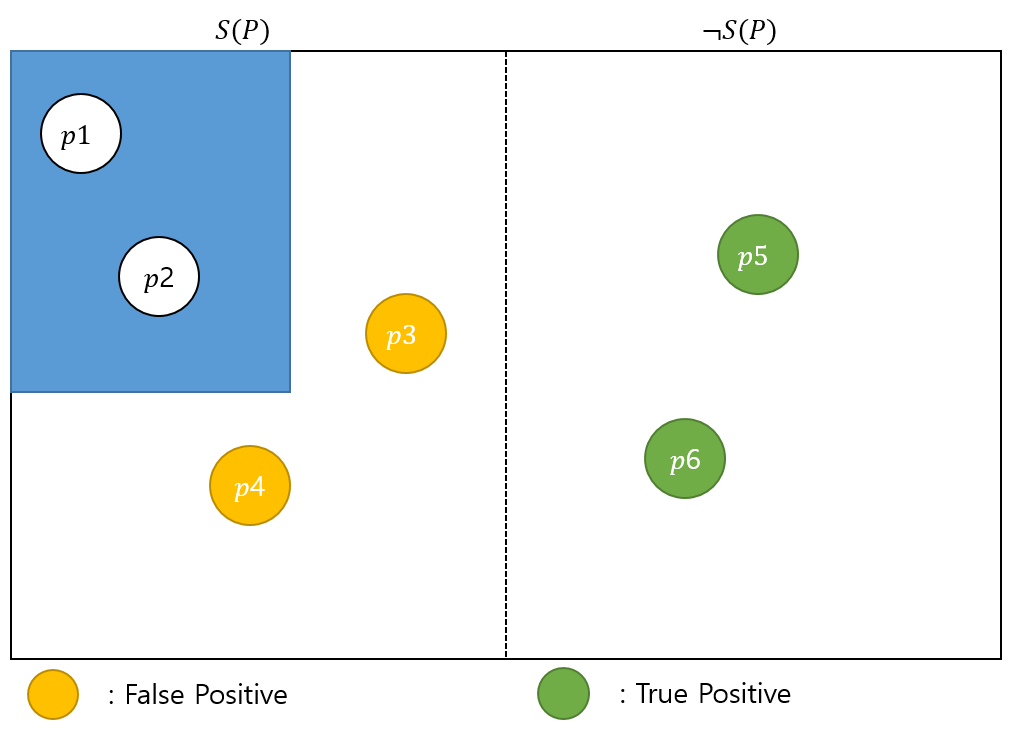
\includegraphics[width=\textwidth]{sound}
  \caption{Sound Analysis}
  \label{fig:sound}
\end{figure}

Figure \ref{fig:sound} shows a sound analysis (the blue area). It
proves correctly for the programs $ p_1 $ and $ p_2 $ that satisfy the
specification ($S(P)$). However, since this analysis is
\textit{incomplete}, it has \textbf{false positives}: it \textbf{does
  not prove} for programs $ p_3 $ and $ p_4 $ that satisfy $S$. In
other words, it proves that $ p_3 $ and $ p_4 $ satisfy $ \neg S(P) $
by emiting \textbf{alarms}, even though they are actually satisfy
$ S(P) $. False positives are also called as \textbf{false alarms}.

\subsection{Completeness}

An analysis is called \textbf{complete} when a program satisfies a
property \textsl{S}, the analysis for that program says that it will
satisfy that property.


\textbf{Complete} but \textbf{unsound} analysis have \textbf{false
  negative}. In other words, it \textbf{wrongly proves} programs that
does not satisfy the property.


\begin{figure}[h]
  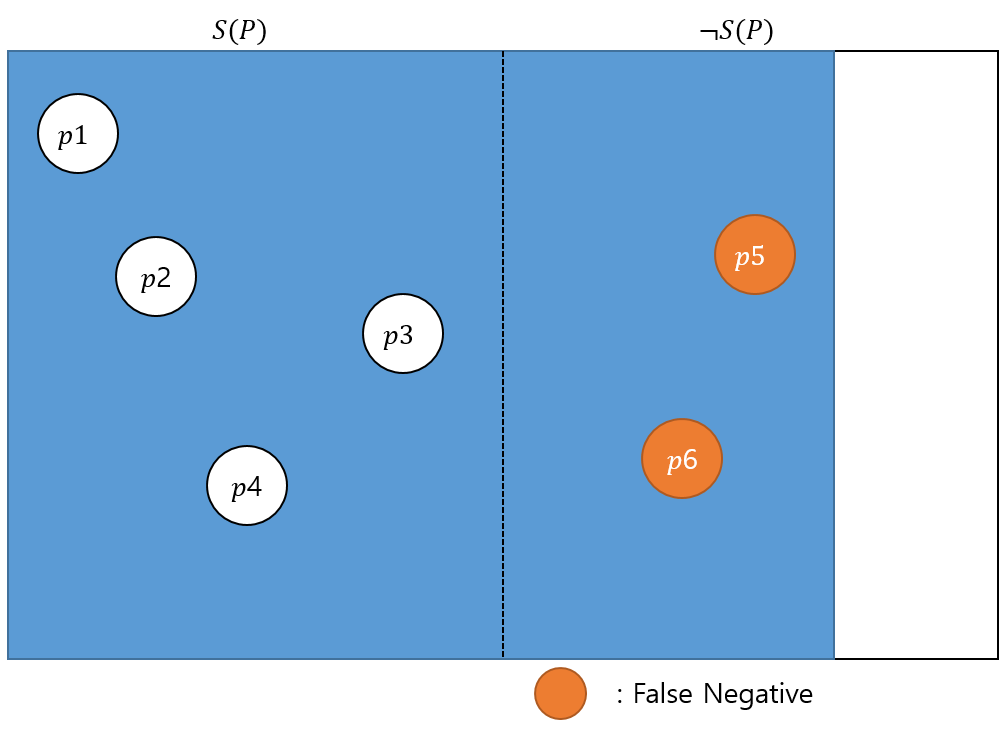
\includegraphics[width=\textwidth]{complete}
  \caption{Complete Analysis}
  \label{fig:complete}
\end{figure}

Figure \ref{fig:complete} shows a complete analysis (also the blue
area). It proves all the programs. In other words, it \textbf{wrongly
  proves} for programs $ p_5 $ and $ p_6 $ that actually do not
satisfy $ S(P) $ by accepting those programs (i.e., emitting no
alarms), thus it is \textit{unsound}. Those programs are \textbf{false
  negatives}.


The table \ref{tab:summary} shows the summary of soundness and
completeness.

\begin{table}[ht]
  \centering
  \caption{Sound \& Complete Summary}
  \label{tab:summary}

  \begin{tabular}[t]{l>{\raggedright}p{0.3\linewidth}>{\raggedright\arraybackslash}p{0.3\linewidth}}
    \hline
    & $ S(P) $ & $ \neg S(P) $ \\
    \hline
    Prove \texttt{(accept)} & \textbf{True negative} (\textsl{correct inference}) & False negative \\
    Not prove \texttt{(reject, alarm)} & False positive & \textbf{True positive} (\textsl{correct inference}) \\
    \hline
  \end{tabular}
\end{table}%


%%% Local Variables:
%%% mode: latex
%%% TeX-master: "program-analysis"
%%% End:
